\documentclass[12pt]{article}
\usepackage[table,xcdraw,dvipsnames]{xcolor}
\usepackage{tabularx}
\usepackage{multirow}
\usepackage{amsmath}
\usepackage{amssymb}
\usepackage{graphicx}
\usepackage{geometry}
\usepackage{setspace}
\usepackage{lipsum}
\usepackage{float}

% Configuración del documento
\geometry{left=2cm, right=2cm, top=2.5cm, bottom=2.5cm}
\setstretch{1.5} % Interlineado

% Centrado global del texto
\makeatletter
\newenvironment{centered}{%
  \begin{center}%
  \let\@currsize\normalsize
  \@currsize
  \vspace{-0.5cm} % Espaciado antes del texto
  \renewcommand{\baselinestretch}{1.5} % Interlineado
  \selectfont}%
  {\end{center}}
\makeatother

\begin{document}

\begin{titlepage}
    \begin{center}
        
        \textbf{\uppercase{Documento de Diseño y Arquitectura de la solución}}\\
        \textbf{Artesanias Bogotá Ltda.}
        
        \vspace{2cm}
        
        \includegraphics[width=0.3\textwidth]{img/ud.png}\\[1cm]
        
            \textbf{Integrantes:}\\[0.5cm]
            Serrano Rodríguez Juan Manuel – 20211020091\\

        \vspace{2cm}
        
            \textbf{Docente:}\\[0.5cm]
            Helio Henry Ramirez Arevalo
        
        \vfill
        
        \textbf{\large{Universidad Distrital Francisco José de Caldas}}\\
        \textbf{\large{Facultad de Ingeniería}}\\
        \textbf{\large{Diseño arquitectural de software y patrones}}\\
        \textbf{\large{Bogotá, 2024}}\\

        
    \end{center}
\end{titlepage}

\tableofcontents
\newpage

\listoffigures
\newpage

\listoftables
\newpage

\section{Descripción del Documento}

\subsection{Propósito y Audiencia}
Este documento tiene como propósito describir la arquitectura de software definida para la plataforma de comercio electrónico Artesanías Bogotá Ltda., orientada a desarrolladores, arquitectos de software y demás interesados en entender la estructura de la aplicación.

\subsection{Organización del Documento}
El documento está dividido en secciones, abordando desde los requerimientos y motivadores arquitecturales hasta los modelos y vistas arquitectónicas de la solución.

\subsection{Convenciones}
Las convenciones en este documento están alineadas con las mejores prácticas de arquitectura de software, siguiendo una organización en capas y basada en eventos.

\subsection{Terminología y Definiciones}
\begin{itemize}
    \item \textbf{Frontend}: Parte de la aplicación accesible y visible para los usuarios. Implementado en Next.js y TypeScript, se encarga de presentar la interfaz gráfica, recibir entradas del usuario y mostrar resultados.
    \item \textbf{Backend}: Capa que contiene la lógica de negocio y las reglas del sistema, desarrollada en Django. Se ocupa de gestionar las operaciones internas, como el procesamiento de pedidos, la gestión de usuarios, y la comunicación con la base de datos y servicios externos.
    \item \textbf{Bull}: Biblioteca de gestión de colas para Node.js que facilita la creación y manejo eficiente de colas de tareas. Permite el procesamiento de trabajos en segundo plano, mejorando la escalabilidad y el rendimiento de la aplicación.
    \item \textbf{Redis}: Sistema de almacenamiento en memoria utilizado como almacenamiento rápido para datos temporales y como backend para Bull. Proporciona alta velocidad en la gestión de colas de tareas y asegura la persistencia necesaria para operaciones asíncronas.
    \item \textbf{PostgreSQL}: Sistema de gestión de bases de datos relacional, utilizado para almacenar los datos estructurados de la plataforma (como productos, usuarios, y pedidos).
    \item \textbf{API REST}: Conjunto de protocolos que define las interacciones entre el frontend y el backend, donde el backend expone funciones para operaciones como el inicio de sesión, la gestión de carritos, y la visualización de productos.
    \item \textbf{E-commerce}: Plataforma digital que permite la compra y venta de productos en línea. En este proyecto, el enfoque de la plataforma es la venta de artesanías de Bogotá, integrando inventarios de puntos de venta físicos.
\end{itemize}

\section{Generalidades del Proyecto}

\subsection{Problema por Resolver}
El problema que se desea resolver es facilitar la compra y gestión de productos artesanales a través de una plataforma en línea, integrando la gestión de inventarios de puntos de venta físicos y el análisis de comportamiento del cliente.

\subsection{Descripción General del Sistema a Desarrollar}
El sistema permite a los usuarios comprar productos artesanales en línea y a los administradores gestionar inventarios en tiempo real y obtener métricas del comportamiento de los usuarios.

\subsection{Objetivos de la Solución}
\begin{itemize}
    \item Desarrollar una plataforma e-commerce para la venta de artesanías.
    \item Integrar la gestión de inventario en tiempo real.
    \item Generar reportes sobre ventas y comportamiento del usuario.
\end{itemize}
\subsection{Stakeholders}

\begin{table}[H]
    \centering
    \begin{tabular}{|p{8cm}|p{8cm}|}
        \hline
        \textbf{Stakeholder} & \textbf{Descripción} \\ \hline
        Administradores de la plataforma & Son responsables de la gestión y configuración general del sitio, así como de la gestión de usuarios y productos. \\ \hline
        Vendedores de Artesanías & Ofrecen sus productos a través de la plataforma. Buscan una plataforma estable y sencilla para publicar, gestionar inventarios y vender productos. \\ \hline
        Clientes & Usuarios que compran productos a través de la plataforma. Buscan una interfaz fácil de usar y confiable para realizar sus compras. \\ \hline
        Equipo de Desarrollo & Desarrolla y mantiene la plataforma. Responsable de implementar y gestionar los componentes técnicos para cumplir con los requisitos del negocio. \\ \hline
        Gerencia General & Define la estrategia y toma decisiones clave de inversión y dirección del proyecto. \\ \hline
    \end{tabular}
    \caption{Stakeholders}
    \label{tab:stakeholders}
\end{table}


\begin{table}[H]
    \centering
    \begin{tabular}{|p{8cm}|p{8cm}|}
        \hline
        \textbf{Stakeholder} & \textbf{Expectativas} \\ \hline
        Administradores de la plataforma & Esperan contar con una plataforma confiable que permita realizar configuraciones y gestionar la base de datos de productos y usuarios sin interrupciones. \\ \hline
        Vendedores de Artesanías & Esperan facilidad para gestionar sus productos y una plataforma que maximice la visibilidad y venta de sus artesanías. \\ \hline
        Clientes & Esperan un sitio seguro, intuitivo y de rápida respuesta para realizar sus compras de manera confiable. \\ \hline
        Equipo de Desarrollo & Espera que la arquitectura sea escalable y mantenible, con una infraestructura que permita desarrollo ágil y la integración de mejoras. \\ \hline
        Gerencia General & Espera que la plataforma apoye el crecimiento del negocio y cumpla con los objetivos de rentabilidad y expansión del mercado. \\ \hline
    \end{tabular}
    \caption{Expectativas de los Stakeholders}
    \label{tab:expectativas_stakeholders}
\end{table}


\section{Especificación y Recabación de Requerimientos Funcionales}
Los requerimientos funcionales son las capacidades específicas que debe cumplir el sistema. Los principales requerimientos son:

\begin{itemize}
    \item \textbf{RF1: Registro e inicio de sesión de usuarios.}
    \item \textbf{RF2: Visualización y búsqueda de productos.}
    \item \textbf{RF3: Gestión de carrito de compras.}
    \item \textbf{RF4: Generación y exportación de reportes de ventas y comportamiento.}
    \item \textbf{RF5: Procesamiento de pagos y confirmación de pedidos.}
\end{itemize}

\subsection{Motivadores de Negocio}
El negocio busca expandir la venta de artesanías a través de una plataforma que permita llegar a más clientes de manera digital y optimizar el manejo de inventario.

\begin{table}[H]
    \centering
    \begin{tabular}{|p{3cm}|p{4cm}|p{4cm}|}
        \hline
        % Nombre del Motivador
        \multicolumn{1}{|>{\columncolor{black}\color{white}}l|}{\textbf{Nombre del Motivador de Negocio}} & 
        \multicolumn{2}{l|}{\cellcolor{black!100}\color{white}\textbf{Descripción del Motivador de Negocio}} \\ \hline
        \multicolumn{1}{|l|}{Expansión de Ventas} & \multicolumn{2}{p{8cm}|}{Ampliar el alcance de mercado para las artesanías, permitiendo a la organización ofrecer productos a nivel nacional e internacional a través de una plataforma digital.}\\ \hline
        
        % Medida del Impacto
        \multicolumn{3}{|>{\columncolor{black}\color{white}}l|}{\textbf{Medida del Impacto}} \\ \hline
        \multicolumn{3}{|l|}{Incremento en las ventas online.} \\ \hline
        
        % Rangos y Cotas
        \multicolumn{1}{|>{\columncolor{black}\color{white}}l|}{\textbf{Rangos}} & 
        \multicolumn{1}{>{\columncolor{black}\color{white}}l|}{\textbf{Cota Mínima}} & 
        \multicolumn{1}{>{\columncolor{black}\color{white}}l|}{\textbf{Cota Máxima}} \\ \hline
        \multicolumn{1}{|>{\columncolor{CadetBlue!30}}l|}{\textbf{Ninguno}}  & & \\ \hline
        \multicolumn{1}{|>{\columncolor{CadetBlue!50}}l|}{\textbf{Bajo}}  & & \\ \hline
        \multicolumn{1}{|>{\columncolor{CadetBlue!70}}l|}{\textbf{Moderado}}  & & \\ \hline
        \multicolumn{1}{|>{\columncolor{CadetBlue!90}}l|}{\textbf{Fuerte}}  &  & \\ \hline
        \multicolumn{1}{|>{\columncolor{CadetBlue!100}}l|}{\textbf{Muy Fuerte}}  & & \\ \hline
        % Asociación del motivador
        \multicolumn{1}{>{\columncolor{black}\color{white}}l|}{\textbf{Asociación del motivador con el negocio}} & 
        \multicolumn{1}{>{\columncolor{black}\color{white}}l|}{\textbf{Definido por:}} & 
        \\ \hline
        \multicolumn{1}{>{\columncolor{black}}l|}{} & \multicolumn{1}{>{\columncolor{black}\color{white}}l|}{\textbf{Ejecutado por:}} & Equipo de Desarrollo \\ \hline
    \end{tabular}
    \caption{Motivadores de Negocio 1}
    \label{tab:motivadores_negocio}
\end{table}

\begin{table}[H]
    \centering
    \begin{tabular}{|p{3cm}|p{4cm}|p{4cm}|}
        \hline
        % Nombre del Motivador
        \multicolumn{1}{|>{\columncolor{black}\color{white}}l|}{\textbf{Nombre del Motivador de Negocio}} & 
        \multicolumn{2}{l|}{\cellcolor{black!100}\color{white}\textbf{Descripción del Motivador de Negocio}} \\ \hline
        \multicolumn{1}{|l|}{Reducción de Costos Operativos} & \multicolumn{2}{p{8cm}|}{Minimizar costos asociados a la gestión de inventarios y ventas físicas al integrar inventarios y reducir la necesidad de puntos de venta físicos.}\\ \hline
        
        % Medida del Impacto
        \multicolumn{3}{|>{\columncolor{black}\color{white}}l|}{\textbf{Medida del Impacto}} \\ \hline
        \multicolumn{3}{|l|}{Ahorro en costos logísticos y operativos.} \\ \hline
        
        % Rangos y Cotas
        \multicolumn{1}{|>{\columncolor{black}\color{white}}l|}{\textbf{Rangos}} & 
        \multicolumn{1}{>{\columncolor{black}\color{white}}l|}{\textbf{Cota Mínima}} & 
        \multicolumn{1}{>{\columncolor{black}\color{white}}l|}{\textbf{Cota Máxima}} \\ \hline
        \multicolumn{1}{|>{\columncolor{CadetBlue!30}}l|}{\textbf{Ninguno}}  & & \\ \hline
        \multicolumn{1}{|>{\columncolor{CadetBlue!50}}l|}{\textbf{Bajo}}  & & \\ \hline
        \multicolumn{1}{|>{\columncolor{CadetBlue!70}}l|}{\textbf{Moderado}}  & & \\ \hline
        \multicolumn{1}{|>{\columncolor{CadetBlue!90}}l|}{\textbf{Fuerte}}  &  & \\ \hline
        \multicolumn{1}{|>{\columncolor{CadetBlue!100}}l|}{\textbf{Muy Fuerte}}  & & \\ \hline
        % Asociación del motivador
        \multicolumn{1}{>{\columncolor{black}\color{white}}l|}{\textbf{Asociación del motivador con el negocio}} & 
        \multicolumn{1}{>{\columncolor{black}\color{white}}l|}{\textbf{Definido por:}} & 
        \\ \hline
        \multicolumn{1}{>{\columncolor{black}}l|}{} & \multicolumn{1}{>{\columncolor{black}\color{white}}l|}{\textbf{Ejecutado por:}} & Administración \\ \hline
    \end{tabular}
    \caption{Motivadores de Negocio 2}
    \label{tab:motivadores_negocio}
\end{table}

\begin{table}[H]
    \centering
    \begin{tabular}{|p{3cm}|p{4cm}|p{4cm}|}
        \hline
        % Nombre del Motivador
        \multicolumn{1}{|>{\columncolor{black}\color{white}}l|}{\textbf{Nombre del Motivador de Negocio}} & 
        \multicolumn{2}{l|}{\cellcolor{black!100}\color{white}\textbf{Descripción del Motivador de Negocio}} \\ \hline
        \multicolumn{1}{|l|}{Mejora de la Experiencia del Cliente} & \multicolumn{2}{p{8cm}|}{Ofrecer una experiencia de usuario intuitiva y amigable que facilite la compra de artesanías, aumente la satisfacción del cliente y genere reseñas positivas.}\\ \hline
        
        % Medida del Impacto
        \multicolumn{3}{|>{\columncolor{black}\color{white}}l|}{\textbf{Medida del Impacto}} \\ \hline
        \multicolumn{3}{|l|}{Incremento en la tasa de conversión y retención de clientes.} \\ \hline
        
        % Rangos y Cotas
        \multicolumn{1}{|>{\columncolor{black}\color{white}}l|}{\textbf{Rangos}} & 
        \multicolumn{1}{>{\columncolor{black}\color{white}}l|}{\textbf{Cota Mínima}} & 
        \multicolumn{1}{>{\columncolor{black}\color{white}}l|}{\textbf{Cota Máxima}} \\ \hline
        \multicolumn{1}{|>{\columncolor{CadetBlue!30}}l|}{\textbf{Ninguno}}  & & \\ \hline
        \multicolumn{1}{|>{\columncolor{CadetBlue!50}}l|}{\textbf{Bajo}}  & & \\ \hline
        \multicolumn{1}{|>{\columncolor{CadetBlue!70}}l|}{\textbf{Moderado}}  & & \\ \hline
        \multicolumn{1}{|>{\columncolor{CadetBlue!90}}l|}{\textbf{Fuerte}}  &  & \\ \hline
        \multicolumn{1}{|>{\columncolor{CadetBlue!100}}l|}{\textbf{Muy Fuerte}}  & & \\ \hline
        % Asociación del motivador
        \multicolumn{1}{>{\columncolor{black}\color{white}}l|}{\textbf{Asociación del motivador con el negocio}} & 
        \multicolumn{1}{>{\columncolor{black}\color{white}}l|}{\textbf{Definido por:}} & 
        \\ \hline
        \multicolumn{1}{>{\columncolor{black}}l|}{} & \multicolumn{1}{>{\columncolor{black}\color{white}}l|}{\textbf{Ejecutado por:}} & Desarrollo (UX/UI) \\ \hline
    \end{tabular}
    \caption{Motivadores de Negocio 3}
    \label{tab:motivadores_negocio}
\end{table}

\subsection{Restricciones de Tecnología}

% Tabla para la restricción RT-01
\begin{table}[H]
    \centering
    \begin{tabular}{|>{\columncolor{teal!50}}l|p{3cm}|p{3cm}|p{3cm}|p{4cm}|}
        \hline
        \textbf{ID Restricción:} & \multicolumn{1}{l|}{RT-01} & \multicolumn{1}{l|}{\cellcolor{teal!50}\begin{tabular}[c]{@{}l@{}}Tipo:\\ (X) Tecnología\\ ( ) Negocio\end{tabular}} & \multicolumn{1}{l|}{\cellcolor{teal!50}Nombre Restricción:} & Uso de PostgreSQL como Base de Datos \\ \hline
        \cellcolor{teal!50}\textbf{Descripción:} & \multicolumn{4}{p{13cm}|}{La base de datos debe ser relacional y normalizada, y PostgreSQL es la elegida por compatibilidad y características avanzadas.} \\ \hline
        \cellcolor{teal!50}\textbf{Establecido por:} & \multicolumn{4}{p{13cm}|}{Equipo de Desarrollo} \\ \hline
        \cellcolor{teal!50}\textbf{Alternativas:} & \multicolumn{4}{p{13cm}|}{MySQL, MariaDB} \\ \hline
        \cellcolor{teal!50}\textbf{Observaciones:} & \multicolumn{4}{p{13cm}|}{PostgreSQL garantiza mayor consistencia de datos para las transacciones críticas de la plataforma.} \\ \hline
    \end{tabular}
    \caption{Restricción de tecnología 1.}
    \label{tab:restricciones_tecnologia}
\end{table}

% Tabla para la restricción RT-02
\begin{table}[H]
    \centering
    \begin{tabular}{|>{\columncolor{teal!50}}l|p{3cm}|p{3cm}|p{3cm}|p{4cm}|}
        \hline
        \textbf{ID Restricción:} & \multicolumn{1}{l|}{RT-02} & \multicolumn{1}{l|}{\cellcolor{teal!50}\begin{tabular}[c]{@{}l@{}}Tipo:\\ (X) Tecnología\\ ( ) Negocio\end{tabular}} & \multicolumn{1}{l|}{\cellcolor{teal!50}Nombre Restricción:} & Herramientas de Mensajería Asíncrona (Bull y Redis) \\ \hline
        \cellcolor{teal!50}\textbf{Descripción:} & \multicolumn{4}{p{13cm}|}{La solución debe ser capaz de manejar eventos de forma asíncrona usando un sistema de colas. Se utilizarán Bull como gestor de colas y Redis como sistema de almacenamiento en memoria.} \\ \hline
        \cellcolor{teal!50}\textbf{Establecido por:} & \multicolumn{4}{p{13cm}|}{Arquitectura de Software} \\ \hline
        \cellcolor{teal!50}\textbf{Alternativas:} & \multicolumn{4}{p{13cm}|}{BullMQ, Bee-Queue} \\ \hline
        \cellcolor{teal!50}\textbf{Observaciones:} & \multicolumn{4}{p{13cm}|}{Bull y Redis se seleccionan por su integración nativa, rendimiento y facilidad de implementación en aplicaciones basadas en eventos.} \\ \hline
    \end{tabular}
    \caption{Restricción de tecnología 2.}
    \label{tab:restricciones_tecnologia_2}
\end{table}

% Tabla para la restricción RB-01
\begin{table}[H]
    \centering
    \begin{tabular}{|>{\columncolor{teal!50}}l|p{3cm}|p{3cm}|p{3cm}|p{4cm}|}
        \hline
        \textbf{ID Restricción:} & \multicolumn{1}{l|}{RB-01} & \multicolumn{1}{l|}{\cellcolor{teal!50}\begin{tabular}[c]{@{}l@{}}Tipo:\\ ( ) Tecnología\\ (X) Negocio\end{tabular}} & \multicolumn{1}{l|}{\cellcolor{teal!50}Nombre Restricción:} & Cumplimiento de Normativa de Protección de Datos \\ \hline
        \cellcolor{teal!50}\textbf{Descripción:} & \multicolumn{4}{p{13cm}|}{La plataforma debe cumplir con regulaciones de privacidad como la GDPR y normas locales para proteger los datos de los usuarios.} \\ \hline
        \cellcolor{teal!50}\textbf{Establecido por:} & \multicolumn{4}{p{13cm}|}{Departamento Legal y Compliance} \\ \hline
        \cellcolor{teal!50}\textbf{Alternativas:} & \multicolumn{4}{p{13cm}|}{No aplicable} \\ \hline
        \cellcolor{teal!50}\textbf{Observaciones:} & \multicolumn{4}{p{13cm}|}{Esto afecta la implementación de medidas de seguridad en la arquitectura, asegurando la protección de datos sensibles y la confidencialidad de las transacciones.} \\ \hline
    \end{tabular}
    \caption{Restricción de negocio 1.}
    \label{tab:restricciones_negocio}
\end{table}

% Tabla para la restricción RB-02
\begin{table}[H]
    \centering
    \begin{tabular}{|>{\columncolor{teal!50}}l|p{3cm}|p{3cm}|p{3cm}|p{4cm}|}
        \hline
        \textbf{ID Restricción:} & \multicolumn{1}{l|}{RB-02} & \multicolumn{1}{l|}{\cellcolor{teal!50}\begin{tabular}[c]{@{}l@{}}Tipo:\\ ( ) Tecnología\\ (X) Negocio\end{tabular}} & \multicolumn{1}{l|}{\cellcolor{teal!50}Nombre Restricción:} & Operatividad en Horario 24/7 \\ \hline
        \cellcolor{teal!50}\textbf{Descripción:} & \multicolumn{4}{p{13cm}|}{La plataforma debe estar disponible 24/7 para todos los usuarios, lo que exige alta disponibilidad y resistencia ante caídas del sistema.} \\ \hline
        \cellcolor{teal!50}\textbf{Establecido por:} & \multicolumn{4}{p{13cm}|}{Gerencia de Operaciones} \\ \hline
        \cellcolor{teal!50}\textbf{Alternativas:} & \multicolumn{4}{p{13cm}|}{Tiempo de mantenimiento nocturno planificado} \\ \hline
        \cellcolor{teal!50}\textbf{Observaciones:} & \multicolumn{4}{p{13cm}|}{La disponibilidad continua de la plataforma es crítica para satisfacer la demanda y asegurar la retención de clientes.} \\ \hline
    \end{tabular}
    \caption{Restricción de negocio 2.}
    \label{tab:restricciones_negocio_2}
\end{table}


\subsection{Atributos de Calidad}
\textbf{Escalabilidad}: La solución debe permitir un crecimiento de usuarios sin afectar el rendimiento. \\
\textbf{Mantenibilidad}: La arquitectura en capas debe permitir modificaciones sin impactar al sistema global. \\
\textbf{Disponibilidad}: Se debe asegurar que el sistema esté operativo al menos el 99\% del tiempo.

\subsection{Recabación y Justificación de Requerimientos No Funcionales}
La solución debe cumplir con los siguientes requerimientos no funcionales, cada uno justificado por la naturaleza y los objetivos del sistema:

\begin{itemize}
    \item \textbf{Escalabilidad}: El sistema debe ser capaz de manejar un aumento en el número de usuarios y productos sin comprometer el rendimiento. Esto se justifica por la posible expansión del negocio, que requiere soportar un tráfico creciente.
    \item \textbf{Disponibilidad}: Se debe asegurar una disponibilidad de al menos el 99\%, garantizando que los usuarios puedan acceder a la plataforma de manera constante. La estabilidad es crítica en plataformas de e-commerce.
    \item \textbf{Seguridad}: Dado que el sistema maneja información sensible, como datos de usuarios y transacciones de pago, se deben implementar mecanismos robustos de autenticación y autorización, además de cumplir con la normativa de protección de datos.
    \item \textbf{Mantenibilidad}: La arquitectura modular y en capas facilita que los desarrolladores puedan hacer cambios o añadir funcionalidades sin afectar otras áreas del sistema.
\end{itemize}

\subsection{Escenarios de Calidad}
Para evaluar el rendimiento y robustez del sistema, se plantean los siguientes escenarios de calidad:

\begin{table}[H]
    \centering
    \begin{tabular}{|p{5cm}|p{3cm}|p{4cm}|p{4cm}|}
        \hline
        \multicolumn{1}{|p{5cm}|}{\cellcolor{teal!50}\textbf{Escenario de Calidad 1:}} & \multicolumn{1}{p{4cm}|}{Alta Disponibilidad} & \multicolumn{1}{l|}{\cellcolor{teal!50}\textbf{Stakeholder:}} & \multicolumn{1}{p{4cm}|}{Administradores de la plataforma} \\ \hline
        \multicolumn{1}{|p{5cm}|}{\cellcolor{teal!50}\textbf{Atributo de Calidad}}    & \multicolumn{3}{p{11cm}|}{Disponibilidad} \\ \hline
        \multicolumn{1}{|p{5cm}|}{\cellcolor{teal!50}\textbf{Justificación}}           & \multicolumn{3}{p{11cm}|}{Los administradores requieren alta disponibilidad para mantener la operación continua y confiable de la plataforma.} \\ \hline
        \multicolumn{1}{|p{5cm}|}{\cellcolor{teal!50}\textbf{Fuente}}                  & \multicolumn{3}{p{11cm}|}{Interacción directa con la plataforma} \\ \hline
        \multicolumn{1}{|p{5cm}|}{\cellcolor{teal!50}\textbf{Estímulo}}                & \multicolumn{3}{p{11cm}|}{Alta demanda de usuarios concurrentes} \\ \hline
        \multicolumn{1}{|p{5cm}|}{\cellcolor{teal!50}\textbf{Artefacto}}               & \multicolumn{3}{p{11cm}|}{Plataforma web completa} \\ \hline
        \multicolumn{1}{|p{5cm}|}{\cellcolor{teal!50}\textbf{Ambiente}}                & \multicolumn{3}{p{11cm}|}{Producción} \\ \hline
        \multicolumn{1}{|p{5cm}|}{\cellcolor{teal!50}\textbf{Respuesta}}               & \multicolumn{3}{p{11cm}|}{Garantizar la disponibilidad continua con redundancia de servidores y balanceo de carga.} \\ \hline
        \multicolumn{1}{|p{5cm}|}{\cellcolor{teal!50}\textbf{Medida de la Respuesta}}  & \multicolumn{3}{p{11cm}|}{Tasa de disponibilidad de 99.9\% anual} \\ \hline
    \end{tabular}
    \caption{Escenario de Calidad 1: Alta Disponibilidad}
    \label{tab:escenarios_calidad_1}
\end{table}


\begin{table}[H]
    \centering
    \begin{tabular}{|p{5cm}|p{3cm}|p{4cm}|p{4cm}|}
        \hline
        \multicolumn{1}{|p{5cm}|}{\cellcolor{teal!50}\textbf{Escenario de Calidad 2:}} & \multicolumn{1}{p{3cm}|}{Facilidad de Uso} & \multicolumn{1}{l|}{\cellcolor{teal!50}\textbf{Stakeholder:}} & \multicolumn{1}{p{4cm}|}{Vendedores de Artesanías} \\ \hline
        \multicolumn{1}{|p{5cm}|}{\cellcolor{teal!50}\textbf{Atributo de Calidad}}    & \multicolumn{3}{p{11cm}|}{Usabilidad} \\ \hline
        \multicolumn{1}{|p{5cm}|}{\cellcolor{teal!50}\textbf{Justificación}}           & \multicolumn{3}{p{11cm}|}{La facilidad de uso permite a los vendedores gestionar sus productos e inventario sin problemas.} \\ \hline
        \multicolumn{1}{|p{5cm}|}{\cellcolor{teal!50}\textbf{Fuente}}                  & \multicolumn{3}{p{11cm}|}{Panel de vendedor de la plataforma} \\ \hline
        \multicolumn{1}{|p{5cm}|}{\cellcolor{teal!50}\textbf{Estímulo}}                & \multicolumn{3}{p{11cm}|}{Interacción frecuente con la interfaz de gestión} \\ \hline
        \multicolumn{1}{|p{5cm}|}{\cellcolor{teal!50}\textbf{Artefacto}}               & \multicolumn{3}{p{11cm}|}{Interfaz de usuario} \\ \hline
        \multicolumn{1}{|p{5cm}|}{\cellcolor{teal!50}\textbf{Ambiente}}                & \multicolumn{3}{p{11cm}|}{Producción} \\ \hline
        \multicolumn{1}{|p{5cm}|}{\cellcolor{teal!50}\textbf{Respuesta}}               & \multicolumn{3}{p{11cm}|}{Interfaz intuitiva y accesible que permita una gestión eficiente.} \\ \hline
        \multicolumn{1}{|p{5cm}|}{\cellcolor{teal!50}\textbf{Medida de la Respuesta}}  & \multicolumn{3}{p{11cm}|}{Reducción del tiempo de gestión a menos de 2 minutos por operación} \\ \hline
    \end{tabular}
    \caption{Escenario de Calidad 2: Facilidad de Uso}
    \label{tab:escenarios_calidad_2}
\end{table}

\begin{table}[H]
    \centering
    \begin{tabular}{|p{5cm}|p{3cm}|p{4cm}|p{4cm}|}
        \hline
        \multicolumn{1}{|p{5cm}|}{\cellcolor{teal!50}\textbf{Escenario de Calidad 3:}} & \multicolumn{1}{p{3cm}|}{Interfaz Intuitiva} & \multicolumn{1}{l|}{\cellcolor{teal!50}\textbf{Stakeholder:}} & \multicolumn{1}{l|}{Clientes} \\ \hline
        \multicolumn{1}{|p{5cm}|}{\cellcolor{teal!50}\textbf{Atributo de Calidad}}    & \multicolumn{3}{p{11cm}|}{Usabilidad} \\ \hline
        \multicolumn{1}{|p{5cm}|}{\cellcolor{teal!50}\textbf{Justificación}}           & \multicolumn{3}{p{11cm}|}{Los clientes requieren una interfaz amigable y fácil de navegar para mejorar la experiencia de usuario.} \\ \hline
        \multicolumn{1}{|p{5cm}|}{\cellcolor{teal!50}\textbf{Fuente}}                  & \multicolumn{3}{p{11cm}|}{Interacción con la plataforma de compra} \\ \hline
        \multicolumn{1}{|p{5cm}|}{\cellcolor{teal!50}\textbf{Estímulo}}                & \multicolumn{3}{p{11cm}|}{Acceso a la plataforma de e-commerce} \\ \hline
        \multicolumn{1}{|p{5cm}|}{\cellcolor{teal!50}\textbf{Artefacto}}               & \multicolumn{3}{p{11cm}|}{Interfaz web de usuario} \\ \hline
        \multicolumn{1}{|p{5cm}|}{\cellcolor{teal!50}\textbf{Ambiente}}                & \multicolumn{3}{p{11cm}|}{Producción} \\ \hline
        \multicolumn{1}{|p{5cm}|}{\cellcolor{teal!50}\textbf{Respuesta}}               & \multicolumn{3}{p{11cm}|}{Ofrecer una interfaz intuitiva y responsive.} \\ \hline
        \multicolumn{1}{|p{5cm}|}{\cellcolor{teal!50}\textbf{Medida de la Respuesta}}  & \multicolumn{3}{p{11cm}|}{Tiempo de respuesta promedio de 2 segundos} \\ \hline
    \end{tabular}
    \caption{Escenario de Calidad 3: Interfaz Intuitiva}
    \label{tab:escenarios_calidad_3}
\end{table}

\begin{table}[H]
    \centering
    \begin{tabular}{|p{5cm}|p{3cm}|p{4cm}|p{4cm}|}
        \hline
        \multicolumn{1}{|p{5cm}|}{\cellcolor{teal!50}\textbf{Escenario de Calidad 4:}} & \multicolumn{1}{p{3cm}|}{Mantenibilidad del Sistema} & \multicolumn{1}{l|}{\cellcolor{teal!50}\textbf{Stakeholder:}} & \multicolumn{1}{l|}{Equipo de Desarrollo} \\ \hline
        \multicolumn{1}{|p{5cm}|}{\cellcolor{teal!50}\textbf{Atributo de Calidad}}    & \multicolumn{3}{p{11cm}|}{Mantenibilidad} \\ \hline
        \multicolumn{1}{|p{5cm}|}{\cellcolor{teal!50}\textbf{Justificación}}           & \multicolumn{3}{p{11cm}|}{La mantenibilidad es crucial para que el equipo de desarrollo realice mejoras y soluciones sin comprometer la estabilidad del sistema.} \\ \hline
        \multicolumn{1}{|p{5cm}|}{\cellcolor{teal!50}\textbf{Fuente}}                  & \multicolumn{3}{p{11cm}|}{Código fuente y documentación} \\ \hline
        \multicolumn{1}{|p{5cm}|}{\cellcolor{teal!50}\textbf{Estímulo}}                & \multicolumn{3}{p{11cm}|}{Cambios en requerimientos o mejoras} \\ \hline
        \multicolumn{1}{|p{5cm}|}{\cellcolor{teal!50}\textbf{Artefacto}}               & \multicolumn{3}{p{11cm}|}{Arquitectura del sistema y código fuente} \\ \hline
        \multicolumn{1}{|p{5cm}|}{\cellcolor{teal!50}\textbf{Ambiente}}                & \multicolumn{3}{p{11cm}|}{Desarrollo y producción} \\ \hline
        \multicolumn{1}{|p{5cm}|}{\cellcolor{teal!50}\textbf{Respuesta}}               & \multicolumn{3}{p{11cm}|}{Documentación clara y modularidad en el código para facilitar cambios.} \\ \hline
        \multicolumn{1}{|p{5cm}|}{\cellcolor{teal!50}\textbf{Medida de la Respuesta}}  & \multicolumn{3}{p{11cm}|}{Tiempo de implementación de cambios dentro del 10\% de desviación} \\ \hline
    \end{tabular}
    \caption{Escenario de Calidad 4: Mantenibilidad del Sistema}
    \label{tab:escenarios_calidad_4}
\end{table}

\begin{table}[H]
    \centering
    \begin{tabular}{|p{5cm}|p{3cm}|p{4cm}|p{4cm}|}
        \hline
        \multicolumn{1}{|p{5cm}|}{\cellcolor{teal!50}\textbf{Escenario de Calidad 5:}} & \multicolumn{1}{p{3cm}|}{Escalabilidad de la Plataforma} & \multicolumn{1}{l|}{\cellcolor{teal!50}\textbf{Stakeholder:}} & \multicolumn{1}{l|}{Gerencia General} \\ \hline
        \multicolumn{1}{|p{5cm}|}{\cellcolor{teal!50}\textbf{Atributo de Calidad}}    & \multicolumn{3}{p{11cm}|}{Escalabilidad} \\ \hline
        \multicolumn{1}{|p{5cm}|}{\cellcolor{teal!50}\textbf{Justificación}}           & \multicolumn{3}{p{11cm}|}{La plataforma debe poder crecer y soportar un aumento en la carga de usuarios y transacciones.} \\ \hline
        \multicolumn{1}{|p{5cm}|}{\cellcolor{teal!50}\textbf{Fuente}}                  & \multicolumn{3}{p{11cm}|}{Crecimiento del negocio y aumento de la demanda} \\ \hline
        \multicolumn{1}{|p{5cm}|}{\cellcolor{teal!50}\textbf{Estímulo}}                & \multicolumn{3}{p{11cm}|}{Incremento en el número de usuarios concurrentes} \\ \hline
        \multicolumn{1}{|p{5cm}|}{\cellcolor{teal!50}\textbf{Artefacto}}               & \multicolumn{3}{p{11cm}|}{Infraestructura del sistema} \\ \hline
        \multicolumn{1}{|p{5cm}|}{\cellcolor{teal!50}\textbf{Ambiente}}                & \multicolumn{3}{p{11cm}|}{Producción} \\ \hline
        \multicolumn{1}{|p{5cm}|}{\cellcolor{teal!50}\textbf{Respuesta}}               & \multicolumn{3}{p{11cm}|}{Aumentar la capacidad de la plataforma mediante infraestructura flexible y escalable.} \\ \hline
        \multicolumn{1}{|p{5cm}|}{\cellcolor{teal!50}\textbf{Medida de la Respuesta}}  & \multicolumn{3}{p{11cm}|}{Capacidad de soporte de un 200\% de incremento en carga sin afectación en desempeño} \\ \hline
    \end{tabular}
    \caption{Escenario de Calidad 5: Escalabilidad de la Plataforma}
    \label{tab:escenarios_calidad_5}
\end{table}


\section{Contexto}
\subsection{Escenarios Operacionales}
El sistema debe permitir la interacción de clientes en la plataforma para navegar, seleccionar productos, y realizar compras, mientras los administradores gestionan productos y reportes.

\begin{table}[H]
    \centering
    \begin{tabular}{|p{4cm}|p{4cm}|p{4cm}|p{4cm}|}
        \hline
        \multicolumn{4}{|l|}{\cellcolor{teal!50}\textbf{Título del Escenario Operacional: Gestión de la Plataforma}} \\ \hline
        \multicolumn{4}{|p{16cm}|}{Los administradores deben tener acceso a herramientas para gestionar usuarios, productos, y configurar la plataforma.} \\ \hline
        \multicolumn{1}{|p{4cm}|}{\cellcolor{teal!50}Stakeholder} & \multicolumn{1}{p{6cm}|}{Administradores de la Plataforma} & \multicolumn{1}{|p{2cm}|}{\cellcolor{teal!50}ID} & \multicolumn{1}{p{4cm}|}{EO-01} \\ \hline
        \multicolumn{1}{|p{4cm}|}{\cellcolor{teal!50}Descripción general de la funcionalidad} & \multicolumn{3}{p{12cm}|}{Permite a los administradores gestionar las configuraciones, productos y usuarios desde un panel de control.} \\ \hline
        \multicolumn{1}{|p{4cm}|}{\cellcolor{teal!50}Describa lo que el stakeholder hace ahora o le gustaría poder hacer} & \multicolumn{3}{p{12cm}|}{Acceder al panel de administración para gestionar datos y operaciones en tiempo real.} \\ \hline
        \multicolumn{1}{|p{4cm}|}{\cellcolor{teal!50}Describa cualquier entrada provista o disponible al momento del inicio} & \multicolumn{3}{p{12cm}|}{Información de usuarios, productos y configuración de la plataforma.} \\ \hline
        \multicolumn{1}{|p{4cm}|}{\cellcolor{teal!50}Describa el contexto de la operación} & \multicolumn{3}{p{12cm}|}{La operación se realiza en un entorno de producción, con conexión a la base de datos y al sistema de mensajería.} \\ \hline
        \multicolumn{1}{|p{4cm}|}{\cellcolor{teal!50}Describa cómo el sistema debe responder} & \multicolumn{3}{p{12cm}|}{El sistema debe responder de manera rápida y precisa a los comandos de administración, actualizando los datos en tiempo real.} \\ \hline
        \multicolumn{1}{|p{4cm}|}{\cellcolor{teal!50}Describa las salidas que el sistema produce como resultado de la acción} & \multicolumn{3}{p{12cm}|}{Reportes de actividad y estado actualizado de configuraciones, usuarios y productos.} \\ \hline
        \multicolumn{1}{|p{4cm}|}{\cellcolor{teal!50}Describa quién o qué usa la salida para qué es utilizada} & \multicolumn{3}{p{12cm}|}{El equipo de administración para monitorear y ajustar operaciones.} \\ \hline
    \end{tabular}
    \caption{Escenario Operacional 1: Gestión de la Plataforma}
    \label{tab:escenario_operacional_1}
\end{table}

\begin{table}[H]
    \centering
    \begin{tabular}{|p{4cm}|p{4cm}|p{4cm}|p{4cm}|}
        \hline
        \multicolumn{4}{|l|}{\cellcolor{teal!50}\textbf{Título del Escenario Operacional: Gestión de Productos}} \\ \hline
        \multicolumn{4}{|p{16cm}|}{Los vendedores pueden gestionar sus productos, inventario y precios en la plataforma para maximizar sus ventas.} \\ \hline
        \multicolumn{1}{|p{4cm}|}{\cellcolor{teal!50}Stakeholder} & \multicolumn{1}{p{6cm}|}{Vendedores de Artesanías} & \multicolumn{1}{|p{2cm}|}{\cellcolor{teal!50}ID} & \multicolumn{1}{p{4cm}|}{EO-02} \\ \hline
        \multicolumn{1}{|p{4cm}|}{\cellcolor{teal!50}Descripción general de la funcionalidad} & \multicolumn{3}{p{12cm}|}{Permitir a los vendedores agregar, editar o eliminar productos desde su panel de gestión.} \\ \hline
        \multicolumn{1}{|p{4cm}|}{\cellcolor{teal!50}Describa lo que el stakeholder hace ahora o le gustaría poder hacer} & \multicolumn{3}{p{12cm}|}{Actualizar información de productos y revisar el inventario en tiempo real.} \\ \hline
        \multicolumn{1}{|p{4cm}|}{\cellcolor{teal!50}Describa cualquier entrada provista o disponible al momento del inicio} & \multicolumn{3}{p{12cm}|}{Datos del producto, como nombre, descripción, precio y cantidad en inventario.} \\ \hline
        \multicolumn{1}{|p{4cm}|}{\cellcolor{teal!50}Describa el contexto de la operación} & \multicolumn{3}{p{12cm}|}{Se realiza en el entorno de producción, interactuando con la base de datos y la capa de negocio.} \\ \hline
        \multicolumn{1}{|p{4cm}|}{\cellcolor{teal!50}Describa cómo el sistema debe responder} & \multicolumn{3}{p{12cm}|}{De manera rápida y precisa para reflejar cambios instantáneamente en la interfaz de usuario.} \\ \hline
        \multicolumn{1}{|p{4cm}|}{\cellcolor{teal!50}Describa las salidas que el sistema produce como resultado de la acción} & \multicolumn{3}{p{12cm}|}{Confirmación de la actualización de productos y registro de cambios en el inventario.} \\ \hline
        \multicolumn{1}{|p{4cm}|}{\cellcolor{teal!50}Describa quién o qué usa la salida para qué es utilizada} & \multicolumn{3}{p{12cm}|}{Los vendedores para monitorear sus productos y ajustar la oferta de acuerdo con la demanda.} \\ \hline
    \end{tabular}
    \caption{Escenario Operacional 2: Gestión de Productos}
    \label{tab:escenario_operacional_2}
\end{table}

\begin{table}[H]
    \centering
    \begin{tabular}{|p{4cm}|p{4cm}|p{4cm}|p{4cm}|}
        \hline
        \multicolumn{4}{|l|}{\cellcolor{teal!50}\textbf{Título del Escenario Operacional: Proceso de Compra}} \\ \hline
        \multicolumn{4}{|p{16cm}|}{Los clientes pueden seleccionar productos y realizar compras de forma segura y eficiente en la plataforma.} \\ \hline
        \multicolumn{1}{|p{4cm}|}{\cellcolor{teal!50}Stakeholder} & \multicolumn{1}{p{6cm}|}{Clientes} & \multicolumn{1}{|p{2cm}|}{\cellcolor{teal!50}ID} & \multicolumn{1}{p{4cm}|}{EO-03} \\ \hline
        \multicolumn{1}{|p{4cm}|}{\cellcolor{teal!50}Descripción general de la funcionalidad} & \multicolumn{3}{p{12cm}|}{Permitir a los clientes buscar productos, agregarlos al carrito y completar la compra.} \\ \hline
        \multicolumn{1}{|p{4cm}|}{\cellcolor{teal!50}Describa lo que el stakeholder hace ahora o le gustaría poder hacer} & \multicolumn{3}{p{12cm}|}{Realizar la compra de manera rápida y sin problemas en cualquier momento.} \\ \hline
        \multicolumn{1}{|p{4cm}|}{\cellcolor{teal!50}Describa cualquier entrada provista o disponible al momento del inicio} & \multicolumn{3}{p{12cm}|}{Productos seleccionados, información de pago y dirección de envío.} \\ \hline
        \multicolumn{1}{|p{4cm}|}{\cellcolor{teal!50}Describa el contexto de la operación} & \multicolumn{3}{p{12cm}|}{Operación en producción con conectividad a la pasarela de pagos y la base de datos.} \\ \hline
        \multicolumn{1}{|p{4cm}|}{\cellcolor{teal!50}Describa cómo el sistema debe responder} & \multicolumn{3}{p{12cm}|}{Respuesta rápida, procesando pagos y generando confirmación de compra.} \\ \hline
        \multicolumn{1}{|p{4cm}|}{\cellcolor{teal!50}Describa las salidas que el sistema produce como resultado de la acción} & \multicolumn{3}{p{12cm}|}{Confirmación de compra y actualización de inventario.} \\ \hline
        \multicolumn{1}{|p{4cm}|}{\cellcolor{teal!50}Describa quién o qué usa la salida para qué es utilizada} & \multicolumn{3}{p{12cm}|}{Clientes y sistema de inventario para gestionar disponibilidad de productos.} \\ \hline
    \end{tabular}
    \caption{Escenario Operacional 3: Proceso de Compra}
    \label{tab:escenario_operacional_3}
\end{table}

\begin{table}[H]
    \centering
    \begin{tabular}{|p{4cm}|p{4cm}|p{4cm}|p{4cm}|}
        \hline
        \multicolumn{4}{|l|}{\cellcolor{teal!50}\textbf{Título del Escenario Operacional: Implementación de Actualizaciones}} \\ \hline
        \multicolumn{4}{|p{16cm}|}{El equipo de desarrollo despliega mejoras y actualizaciones al sistema sin interrumpir la operación.} \\ \hline
        \multicolumn{1}{|p{4cm}|}{\cellcolor{teal!50}Stakeholder} & \multicolumn{1}{p{6cm}|}{Equipo de Desarrollo} & \multicolumn{1}{|p{2cm}|}{\cellcolor{teal!50}ID} & \multicolumn{1}{p{4cm}|}{EO-04} \\ \hline
        \multicolumn{1}{|p{4cm}|}{\cellcolor{teal!50}Descripción general de la funcionalidad} & \multicolumn{3}{p{12cm}|}{Habilitar a los desarrolladores para realizar actualizaciones del sistema y correcciones de errores.} \\ \hline
        \multicolumn{1}{|p{4cm}|}{\cellcolor{teal!50}Describa lo que el stakeholder hace ahora o le gustaría poder hacer} & \multicolumn{3}{p{12cm}|}{Ejecutar despliegues sin afectar la disponibilidad para los usuarios finales.} \\ \hline
        \multicolumn{1}{|p{4cm}|}{\cellcolor{teal!50}Describa cualquier entrada provista o disponible al momento del inicio} & \multicolumn{3}{p{12cm}|}{Código fuente actualizado y documentación de cambios.} \\ \hline
        \multicolumn{1}{|p{4cm}|}{\cellcolor{teal!50}Describa el contexto de la operación} & \multicolumn{3}{p{12cm}|}{Entorno de producción, con control de versiones y pruebas automatizadas.} \\ \hline
        \multicolumn{1}{|p{4cm}|}{\cellcolor{teal!50}Describa cómo el sistema debe responder} & \multicolumn{3}{p{12cm}|}{Mantener estabilidad mientras se aplican las actualizaciones sin interrupciones.} \\ \hline
        \multicolumn{1}{|p{4cm}|}{\cellcolor{teal!50}Describa las salidas que el sistema produce como resultado de la acción} & \multicolumn{3}{p{12cm}|}{Actualización exitosa y registro de cambios en la versión.} \\ \hline
        \multicolumn{1}{|p{4cm}|}{\cellcolor{teal!50}Describa quién o qué usa la salida para qué es utilizada} & \multicolumn{3}{p{12cm}|}{Equipo de desarrollo para futuras referencias y mejora continua.} \\ \hline
    \end{tabular}
    \caption{Escenario Operacional 4: Implementación de Actualizaciones}
    \label{tab:escenario_operacional_4}
\end{table}

\begin{table}[H]
    \centering
    \begin{tabular}{|p{4cm}|p{4cm}|p{4cm}|p{4cm}|}
        \hline
        \multicolumn{4}{|l|}{\cellcolor{teal!50}\textbf{Título del Escenario Operacional: Monitoreo de Rendimiento}} \\ \hline
        \multicolumn{4}{|p{16cm}|}{La gerencia puede acceder a informes y métricas de rendimiento para la toma de decisiones estratégicas.} \\ \hline
        \multicolumn{1}{|p{4cm}|}{\cellcolor{teal!50}Stakeholder} & \multicolumn{1}{p{6cm}|}{Gerencia General} & \multicolumn{1}{|p{2cm}|}{\cellcolor{teal!50}ID} & \multicolumn{1}{p{4cm}|}{EO-05} \\ \hline
        \multicolumn{1}{|p{4cm}|}{\cellcolor{teal!50}Descripción general de la funcionalidad} & \multicolumn{3}{p{12cm}|}{Acceso a datos sobre transacciones, visitas y rendimiento del sistema en un tablero de control.} \\ \hline
        \multicolumn{1}{|p{4cm}|}{\cellcolor{teal!50}Describa lo que el stakeholder hace ahora o le gustaría poder hacer} & \multicolumn{3}{p{12cm}|}{Revisar los informes y métricas de rendimiento para evaluar el estado del negocio.} \\ \hline
        \multicolumn{1}{|p{4cm}|}{\cellcolor{teal!50}Describa cualquier entrada provista o disponible al momento del inicio} & \multicolumn{3}{p{12cm}|}{Datos de ventas, tráfico y métricas de la plataforma.} \\ \hline
        \multicolumn{1}{|p{4cm}|}{\cellcolor{teal!50}Describa el contexto de la operación} & \multicolumn{3}{p{12cm}|}{Entorno de producción con acceso seguro a la base de datos y sistema de reportes.} \\ \hline
        \multicolumn{1}{|p{4cm}|}{\cellcolor{teal!50}Describa cómo el sistema debe responder} & \multicolumn{3}{p{12cm}|}{Proveer reportes y estadísticas en tiempo real de forma confiable.} \\ \hline
        \multicolumn{1}{|p{4cm}|}{\cellcolor{teal!50}Describa las salidas que el sistema produce como resultado de la acción} & \multicolumn{3}{p{12cm}|}{Reportes y gráficos sobre rendimiento y métricas clave.} \\ \hline
        \multicolumn{1}{|p{4cm}|}{\cellcolor{teal!50}Describa quién o qué usa la salida para qué es utilizada} & \multicolumn{3}{p{12cm}|}{Gerencia para toma de decisiones estratégicas.} \\ \hline
    \end{tabular}
    \caption{Escenario Operacional 5: Monitoreo de Rendimiento}
    \label{tab:escenario_operacional_5}
\end{table}


\subsection{Casos de Uso: Descripción y Modelo}
A continuación se describen los principales casos de uso:
\begin{itemize}
    \item \textbf{UC01: Registro de Usuarios} - El usuario crea una cuenta en la plataforma proporcionando sus datos. La cuenta será validada y almacenada en la base de datos.
    \item \textbf{UC02: Iniciar Sesión} - Permite a los usuarios registrados acceder a sus cuentas usando credenciales. En caso de autenticación exitosa, el usuario obtiene acceso a la plataforma.
    \item \textbf{UC03: Buscar Producto} - El usuario realiza búsquedas de productos en la plataforma mediante un campo de búsqueda que devuelve resultados relevantes.
    \item \textbf{UC04: Agregar al Carrito} - Los usuarios pueden añadir productos al carrito de compras para continuar con el proceso de compra.
    \item \textbf{UC05: Eliminar del Carrito} - Permite a los usuarios quitar productos del carrito antes de confirmar la compra.
    \item \textbf{UC06: Realizar Compra} - Los usuarios finalizan la compra de los productos en el carrito, seleccionando el método de pago y proporcionando la información necesaria.
    \item \textbf{UC07: Calificar Producto} - Luego de la compra, el usuario puede calificar y comentar sobre los productos adquiridos.
    \item \textbf{UC08: Crear Producto (Administrador)} - Los administradores pueden agregar nuevos productos al inventario disponible en la plataforma.
    \item \textbf{UC09: Editar Producto (Administrador)} - Permite que los administradores editen la información de productos ya registrados.
    \item \textbf{UC10: Eliminar Producto (Administrador)} - Los administradores pueden eliminar productos del catálogo de la plataforma.
    \item \textbf{UC11: Generar Reportes} - Permite al administrador crear y exportar reportes de ventas, inventario, y comportamiento de usuarios.
\end{itemize}

\section{Descripción y Justificación de la Arquitectura de Software Definida}

La arquitectura del sistema se basa en un estilo de arquitectura en capas, complementado con una orientación hacia eventos distribuidos para soportar tareas asíncronas.

\begin{itemize}
    \item \textbf{Arquitectura en Capas} - La organización en capas permite separar la lógica de presentación, negocio y datos. Esto facilita la mantenibilidad y la escalabilidad del sistema al permitir que cada capa pueda ser desarrollada y mantenida de manera independiente.
    \item \textbf{Arquitectura Basada en Eventos} - Se emplean Bull y Redis para la gestión de colas y el almacenamiento en memoria. Este estilo arquitectural permite que el sistema responda eficientemente a acciones que no requieren procesamiento inmediato, como actualizaciones de inventario y confirmaciones de pedidos.

    \subsection{Descripción específica de la arquitectura}

    \subsubsection{Capa de Presentación (Frontend - Next.js con TypeScript)}
    \textbf{Descripción:} El frontend, implementado en Next.js con TypeScript, maneja la interacción directa con el usuario, proporcionando una interfaz visual donde se pueden navegar y visualizar productos, agregar elementos al carrito, realizar pagos y calificar productos.

    \textbf{Componentes:}
    \begin{itemize}
        \item \textbf{Páginas de usuario:} Registro, inicio de sesión, perfil de usuario.
        \item \textbf{Catálogo de productos:} Vista de productos, búsqueda, detalles de productos.
        \item \textbf{Carrito de compras:} Gestión de productos añadidos y proceso de checkout.
        \item \textbf{Interacción con el backend:} Las peticiones HTTP se realizan a través de API REST hacia el backend, utilizando Axios u otra librería para la comunicación HTTP.
        \item \textbf{Interacción con Bull y Redis:} Next.js no se comunica directamente con Bull y Redis, pero visualiza el estado actualizado tras la confirmación de los eventos procesados en el backend.
    \end{itemize}

    \subsubsection{Capa de Negocio (Backend - Strapi)}
    \textbf{Descripción:} La capa de negocio está compuesta por un backend en Strapi que gestiona la lógica de negocio y maneja la mayor parte de la funcionalidad crítica del sistema.

    \textbf{Componentes:}
    \begin{itemize}
        \item \textbf{API RESTful:} Strapi expone APIs que permiten el acceso a datos y funcionalidades del sistema para el frontend. Las APIs incluyen:
        \begin{itemize}
            \item \textbf{Autenticación:} Manejo de usuarios y autenticación.
            \item \textbf{Gestión de productos:} Endpoints CRUD para visualizar, agregar, editar y eliminar productos.
            \item \textbf{Carrito de compras:} Endpoints para gestionar los productos en el carrito.
            \item \textbf{Pedidos y Pagos:} Gestión del procesamiento de pagos y confirmación de pedidos.
            \item \textbf{Reportes:} Generación y exportación de reportes en formatos como PDF o Excel.
        \end{itemize}
        \item \textbf{Eventos y Comunicación Asíncrona:} Strapi utiliza Bull para gestionar tareas asíncronas en función de acciones del usuario. Por ejemplo:
        \begin{itemize}
            \item Actualización de inventario al realizar una compra.
            \item Envío de correos de confirmación después del pago.
        \end{itemize}
        \item \textbf{Integración con Bull y Redis:} Strapi se integra con Bull para la gestión de colas de tareas asíncronas, y Redis actúa como sistema de almacenamiento en memoria para estas colas. Esto permite manejar tareas que requieren procesamiento en segundo plano sin afectar la experiencia del usuario.
    \end{itemize}

    \subsubsection{Capa de Persistencia (Base de Datos - PostgreSQL)}
    \textbf{Descripción:} PostgreSQL es la base de datos relacional que almacena toda la información estructurada del sistema.

    \textbf{Componentes:}
    \begin{itemize}
        \item \textbf{Tablas de usuarios, productos, pedidos, inventario, reportes y reseñas:} Estas tablas están normalizadas para mejorar la eficiencia y asegurar la consistencia de los datos.
        \item \textbf{Conexión mediante ORM de Strapi:} Strapi utiliza su propio ORM para interactuar con PostgreSQL, lo que permite manipular datos a través de modelos definidos en el CMS.
        \item \textbf{Integridad de los datos:} La base de datos asegura que los datos de pedidos, inventarios y usuarios permanezcan consistentes, incluso si fallan los procesos de tareas asíncronas.
    \end{itemize}

    \subsubsection{Capa de Integración de Mensajería (Bull y Redis)}
    \textbf{Descripción:} Bull y Redis forman la infraestructura de comunicación basada en eventos y el procesamiento de tareas asíncronas.

    \textbf{Componentes:}
    \begin{itemize}
        \item \textbf{Redis (Almacenamiento en Memoria):} Actúa como almacenamiento rápido para datos temporales y como backend para Bull. Proporciona alta velocidad en la gestión de colas de tareas y asegura la persistencia necesaria para operaciones asíncronas.
        \item \textbf{Bull (Gestor de Colas de Tareas):} Bull facilita la creación y manejo eficiente de colas de tareas. Permite el procesamiento de trabajos en segundo plano, mejorando la escalabilidad y el rendimiento de la aplicación.
        \item \textbf{Gestión de Errores y Reintentos:} Bull maneja los errores en la ejecución de tareas, permitiendo reintentos automáticos en caso de fallos de procesamiento.
    \end{itemize}
\end{itemize}

\subsubsection{Diagrama de Arquitectura}
\begin{figure}[H]
    \centering
    \includegraphics[width=\textwidth]{img/DiagramaArquitectura.pdf}
    \caption{Diagrama de Arquitectura}
    \label{fig:diagrama_arquitectura}
\end{figure}

\section{Descripción y Justificación del (los) Patrón(es) de Diseño Adoptado(s)}

\subsection{Patrón Observador (Observer)}
\textbf{Descripción y Justificación:} El patrón Observador permite que uno o varios objetos (observadores) se suscriban a un objeto principal (sujeto) y reciban notificaciones cuando ocurren cambios. En una arquitectura de eventos, este patrón es útil para permitir la comunicación asíncrona entre componentes.

\textbf{Uso en el Proyecto:} En este caso, el backend (Strapi) actúa como el sujeto, y Bull actúa como el observador que procesa los eventos generados.

\textbf{Implementación:}
\begin{itemize}
    \item Cuando un usuario realiza una compra, el backend genera un evento “pedido confirmado” y lo envía a Bull.
    \item Bull, como observador, está a la escucha y procesa el evento, actualizando el inventario y enviando una confirmación al usuario.
\end{itemize}

\textbf{Beneficio:} Permite un flujo de trabajo sin bloqueo, en el cual los consumidores procesan tareas en segundo plano sin interrumpir la experiencia del usuario.

\subsection{Patrón Mediador (Mediator)}
\textbf{Descripción y Justificación:} El Mediador coordina la comunicación entre diferentes componentes para reducir dependencias directas. En este proyecto, Bull actúa como el mediador que distribuye eventos entre los componentes sin que interactúen directamente entre sí.

\textbf{Uso en el Proyecto:} Bull actúa como mediador entre Strapi y los servicios de procesamiento de tareas, manejando la comunicación de eventos y asegurando que las tareas se enruten correctamente.

\textbf{Implementación:}
\begin{itemize}
    \item Strapi envía un mensaje a Bull cuando se realiza un pedido.
    \item Bull distribuye el mensaje a los consumidores correspondientes, que procesan las tareas necesarias.
\end{itemize}

\textbf{Beneficio:} Elimina dependencias directas entre componentes, lo cual hace que el sistema sea más flexible y escalable al permitir la adición de nuevos consumidores sin modificar el backend.

\subsection{Patrón Fábrica (Factory)}
\textbf{Descripción y Justificación:} El patrón Fábrica permite la creación de objetos complejos sin especificar la clase exacta del objeto que se creará. Este patrón es útil cuando tienes diferentes tipos de productos o usuarios que comparten algunas propiedades comunes.

\textbf{Uso en el Proyecto:} La fábrica puede encargarse de crear diferentes tipos de productos con atributos específicos según sus categorías.

\textbf{Implementación:}
\begin{itemize}
    \item Un “ProductoFactory” puede recibir un tipo de producto (por ejemplo, “artesanía textil” o “cerámica”) y devolver un objeto con los atributos específicos de cada tipo.
\end{itemize}

\textbf{Beneficio:} Centraliza la creación de objetos, lo que permite un manejo más estructurado y facilita el mantenimiento si se necesita cambiar la lógica de creación de productos en el futuro.

\subsection{Patrón Fachada (Facade)}
\textbf{Descripción y Justificación:} La Fachada proporciona una interfaz simplificada para un sistema complejo, lo que permite que otros componentes interactúen con él sin conocer su estructura interna.

\textbf{Uso en el Proyecto:} Strapi puede utilizar controladores de rutas que actúen como una fachada, exponiendo solo los endpoints necesarios para el frontend, simplificando así la interacción.

\textbf{Implementación:}
\begin{itemize}
    \item Un controlador de rutas en Strapi que ofrece los endpoints para la gestión de usuarios, el carrito y los pedidos actúa como una fachada, ocultando la lógica compleja de negocio y acceso a datos.
\end{itemize}

\textbf{Beneficio:} Facilita el mantenimiento del backend al exponer solo lo necesario y ocultar los detalles complejos de la lógica de negocio.

\subsection{Patrón Repositorio (Repository)}
\textbf{Descripción y Justificación:} El patrón de Repositorio proporciona una capa de abstracción entre la lógica de negocio y la capa de acceso a datos. Esto ayuda a organizar y reutilizar el acceso a datos de forma eficiente.

\textbf{Uso en el Proyecto:} En Strapi, el patrón de repositorio se puede implementar encapsulando consultas complejas en servicios que gestionan la interacción con PostgreSQL.

\textbf{Implementación:}
\begin{itemize}
    \item Un servicio de productos puede ofrecer métodos específicos, como obtenerProductosPorCategoría o actualizarInventario, que interactúan con el ORM de Strapi y encapsulan la lógica de consulta de datos.
\end{itemize}

\textbf{Beneficio:} Simplifica el acceso a datos y mantiene la lógica de negocio desacoplada del acceso directo a la base de datos, lo que facilita la adaptación del código a cambios en la estructura de datos.

\subsection{Patrón Singleton}
\textbf{Descripción y Justificación:} El patrón Singleton garantiza que una clase tenga una única instancia y proporciona un punto de acceso global a ella. Es ideal para recursos que deben ser únicos en la aplicación.

\textbf{Uso en el Proyecto:} Este patrón se puede aplicar a la configuración de conexión de la base de datos o a la configuración de Bull en el backend.

\textbf{Implementación:}
\begin{itemize}
    \item La instancia de conexión a la base de datos puede ser un Singleton, asegurando que Strapi utilice siempre la misma conexión, lo que reduce el uso de recursos.
\end{itemize}

\textbf{Beneficio:} Evita la duplicación de instancias para recursos críticos, ahorra memoria y simplifica el acceso a configuraciones compartidas en diferentes partes del sistema.
\section{Puntos de Vista y Modelos Arquitecturales}

\subsection{Punto de Vista: Descripción del Problema}
\subsubsection{Punto de Vista: Contexto de la Solución (Diagrama de Contexto)}
\begin{figure}[H]
    \centering
    \includegraphics[width=\textwidth]{img/Diagrama de contexto.pdf}
    \caption{Diagrama de Contexto}
    \label{fig:diagrama_contexto}
\end{figure}

\subsubsection{Punto de Vista: Objetos (Diagrama de Objetos)}
\begin{figure}[H]
    \centering
    \caption{Diagrama de Objetos}
    \includegraphics[width=\textwidth]{img/DiagramaObjetos.pdf}
    \label{fig:diagrama_objetos}
\end{figure}

\subsection{Punto de Vista: Interacción}

\subsubsection{Diagrama de Casos de Uso}
\begin{figure}[H]
    \centering
    \includegraphics[width=\textwidth]{img/CasosDeUso.jpg}
    \caption{Diagrama de Casos de Uso}
    \label{fig:diagrama_casos_uso}
\end{figure}

\subsubsection{Diagrama de Secuencia}
\begin{figure}[H]
    \centering
    \includegraphics[width=\textwidth]{img/DiagramaSecuencia.pdf}
    \caption{Diagrama de Secuencia}
    \label{fig:diagrama_secuencia}
\end{figure}

\subsection{Punto de Vista: Funcional (Diagrama de Componentes)}
\begin{figure}[H]
    \centering
    \includegraphics[width=\textwidth]{img/DiagramaComponentes.pdf}
    \caption{Diagrama de Componentes}
    \label{fig:diagrama_componentes}
\end{figure}

\subsection{Punto de Vista: Despliegue (Diagrama de Despliegue)}
\begin{figure}[H]
    \centering
    \includegraphics[width=\textwidth]{img/ud.png}
    \caption{Diagrama de Despliegue}
    \label{fig:diagrama_despliegue}
\end{figure}

\subsection{Punto de Vista: Información (Diagrama(s) de Actividades)}
\begin{figure}[H]
    \centering
    \includegraphics[width=0.5\textwidth]{img/DiagramaActividades.pdf}
    \caption{Diagrama de Actividades}
    \label{fig:diagrama_actividades}
\end{figure}

\subsection{Punto de Vista: Desarrollo (Diagrama de Clases)}

\begin{figure}[H]
    \centering
    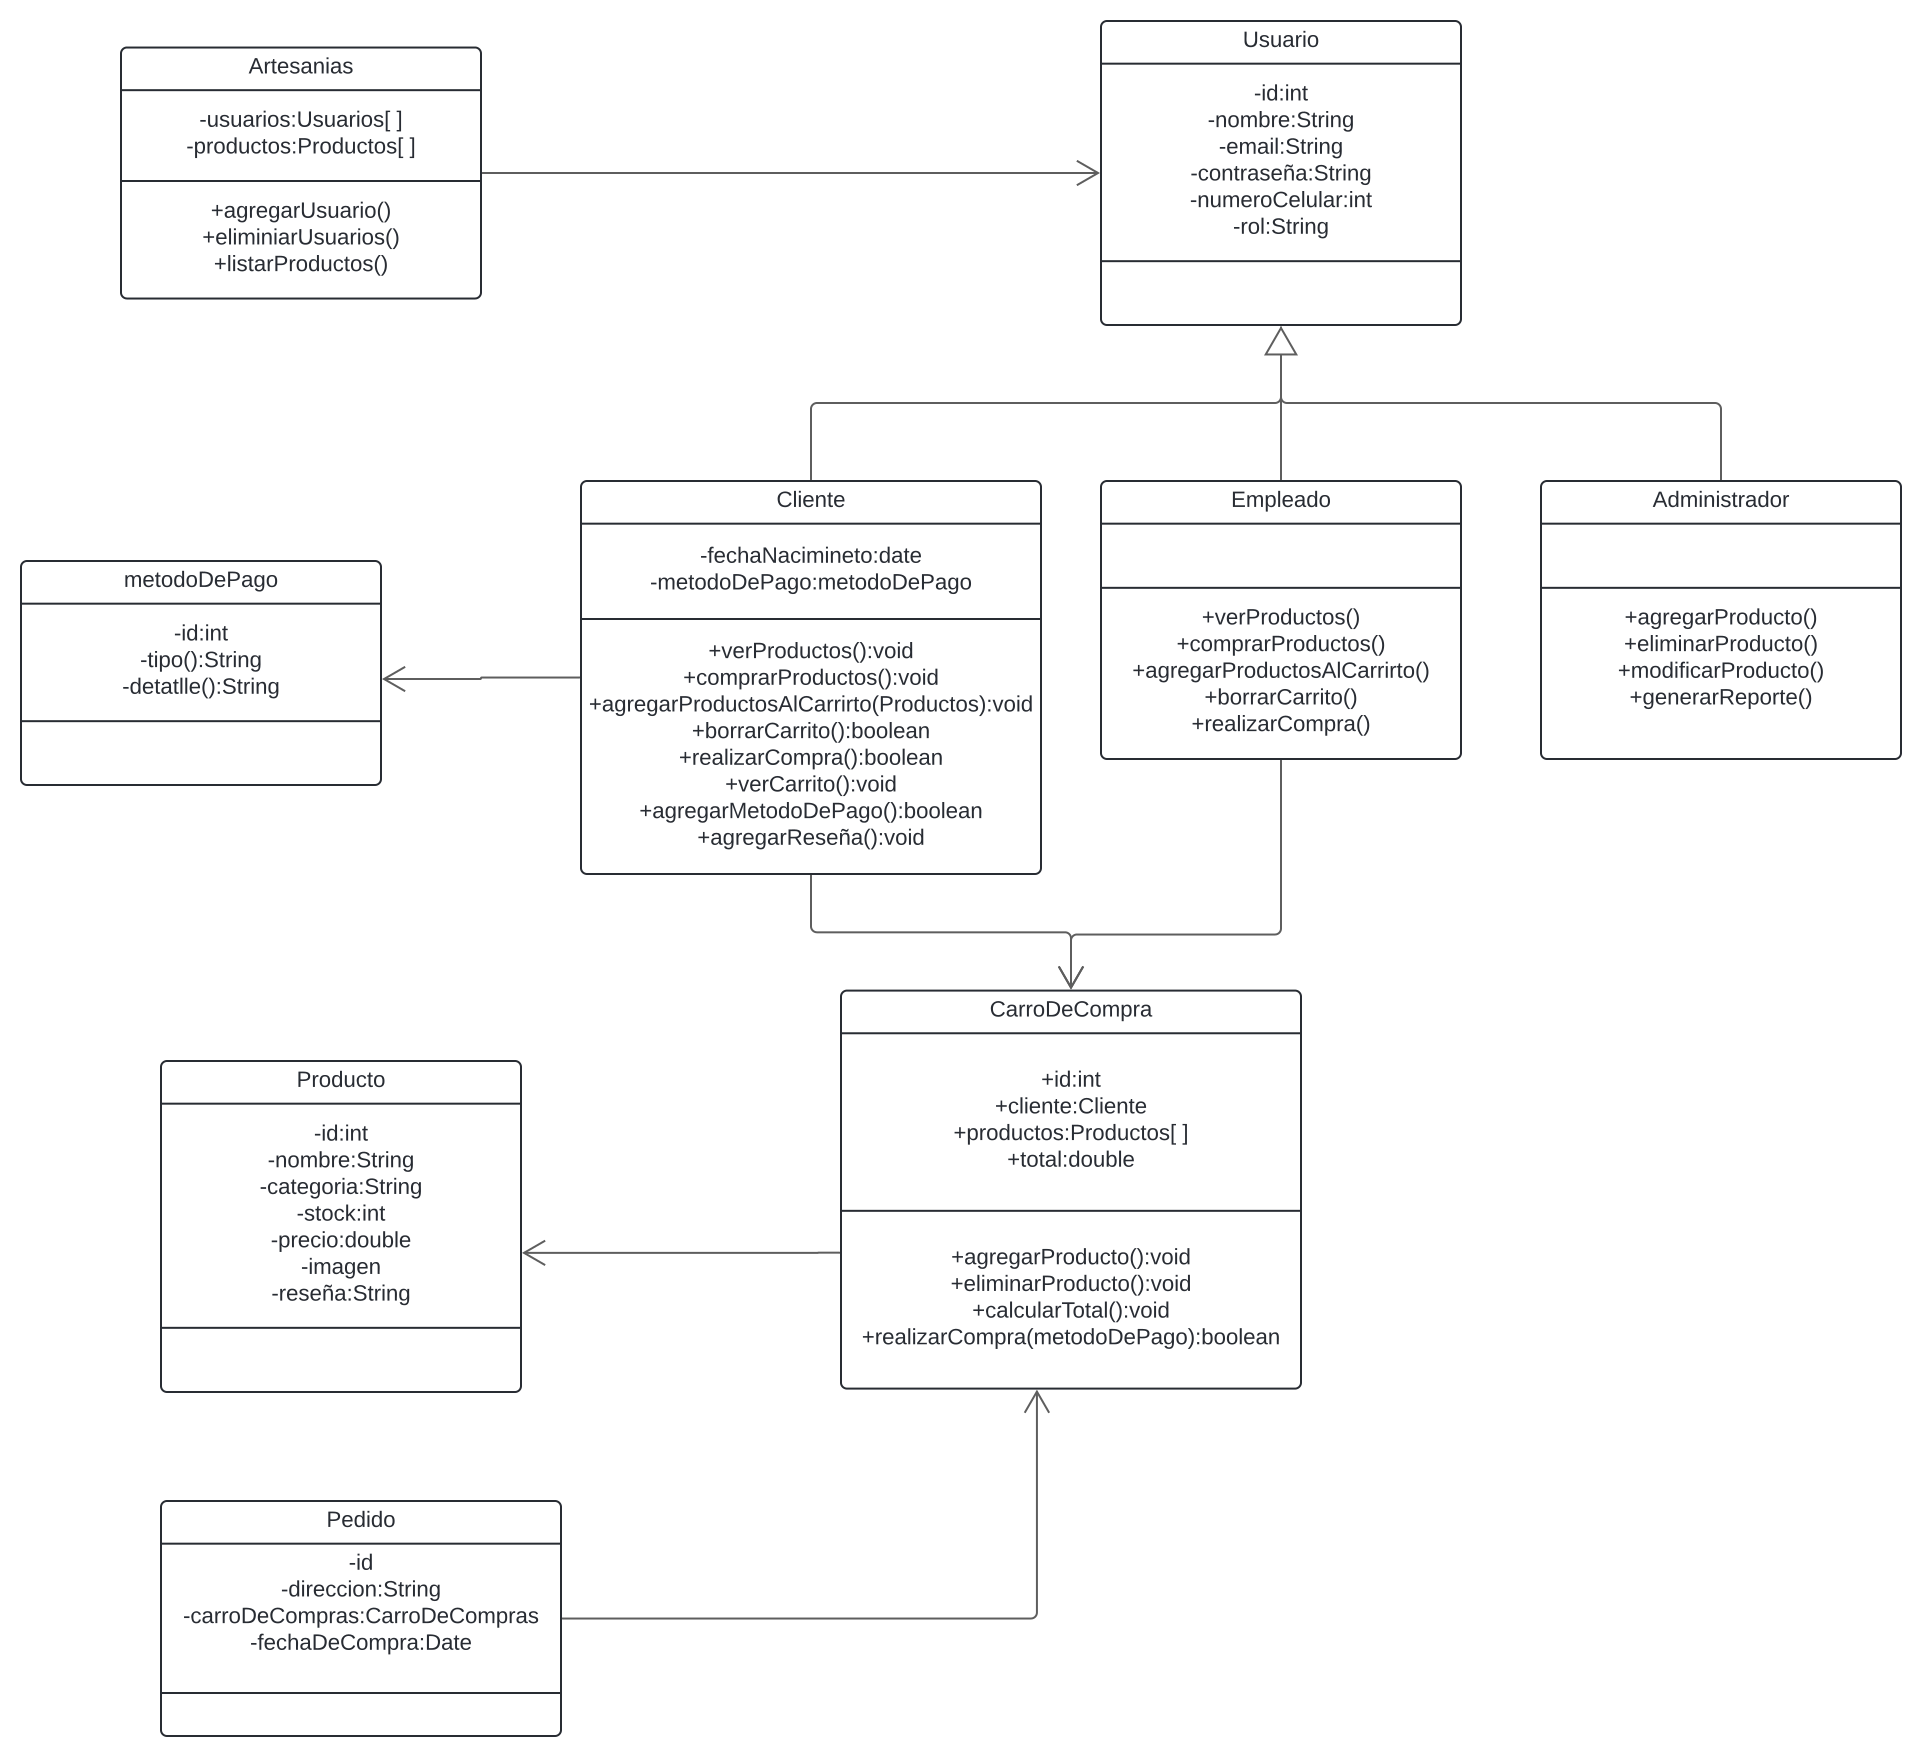
\includegraphics[width=\textwidth]{img/DiagramaClases.pdf}
    \caption{Diagrama de Clases}
    \label{fig:diagrama_clases}
\end{figure}

\subsection{Punto de Vista: Modelo Relacional de la BBDD}
\begin{figure}[H]
    \centering
    \includegraphics[width=\textwidth]{img/ud.png}
    \caption{Modelo Relacional de la BBDD}
    \label{fig:modelo_relacional}
\end{figure}

\section{Justificación y Relaciones entre los Puntos de Vista}
asd

\section{Firmas de Aceptación}
\begin{itemize}
    \item Firma 1: \_\_\_\_\_\_\_\_\_\_\_\_\_\_\_\_\_\_\_\_\_ Fecha: DD/MM/AAAA
    \item Firma 2: \_\_\_\_\_\_\_\_\_\_\_\_\_\_\_\_\_\_\_\_\_ Fecha: DD/MM/AAAA
    \item Firma 3: \_\_\_\_\_\_\_\_\_\_\_\_\_\_\_\_\_\_\_\_\_ Fecha: DD/MM/AAAA
    \item Firma 4: \_\_\_\_\_\_\_\_\_\_\_\_\_\_\_\_\_\_\_\_\_ Fecha: DD/MM/AAAA
    \item Firma 5: \_\_\_\_\_\_\_\_\_\_\_\_\_\_\_\_\_\_\_\_\_ Fecha: DD/MM/AAAA
    \item Firma 6: \_\_\_\_\_\_\_\_\_\_\_\_\_\_\_\_\_\_\_\_\_ Fecha: DD/MM/AAAA
\end{itemize}

\bibliographystyle{plain}
\bibliography{bibliografia}

\end{document}